
Code at \url{https://github.com/cedrict/fieldstone/tree/master/python_codes/fieldstone_64}

%.......................................................
\paragraph{Stress build-up in viscoelastic Maxwell body}

The first benchmark performed to test the viscoelastic implementation considers the stress 
build-up present in a viscoelastic Maxwell body. Contrary to stressed viscous materials, 
viscoelastic materials gradually build-up stress when sheared after which a transition to viscous deformation occurs.  

An unstressed, incompressible viscoelastic Maxwell medium is subjected to a velocity field 
resulting in pure shear. 
The increase of the accumulated stress with time is given by an analytical solution:
\begin{equation}
{\bm \tau} = 2\eta\ {\dot{\bm \varepsilon}} \left ( 1-e^{\frac{-\mu }{\eta} t } \right )
\end{equation}
with $t$ time, $\eta$ the prescribed material viscosity and $\mu$ the prescribed material shear modulus. 
The domain size is 100$\times 100$km.
The velocity prescribed at all boundaries equals $v=1$ cm/yr in magnitude yielding a constant 
background strain rate of $\dot{\varepsilon}=2\text{cm/yr}/100\text{km}\simeq 6.342\times 10^{-15}$. 
The viscosity is $\eta= 10^{21}\text{Pa.s}$, the shear modulus is 
$\mu =10^{10}$Pa and the gravity is set to zero. We set $\delta t=100$yr.  

\begin{center}
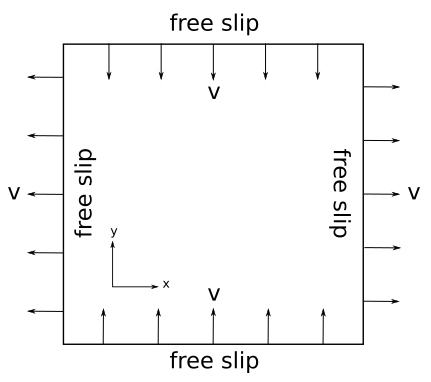
\includegraphics[width=5cm]{python_codes/fieldstone_64/images/stress_buildup_setup.png}\\
\captionfont{
Set up of the stress build-up benchmark. All domain sides have a free slip
boundary condition, and pure shear velocity conditions are prescribed. Adapted from 
Gerya (2010) \cite{gery10}.} 
\end{center}

We have 
\[
\eta_{eff} 
= \frac{\eta \delta t}{\delta t + \eta/\mu} 
= \frac{10^{21} \cdot 3.154\times 10^{9}}{3.154\times 10^{9} + 10^{21}/10^{10}} 
\simeq 
3.057\times 10^{19}\text{Pa.s}
\qquad
\text{and}
\qquad
Z=\frac{\eta_{eff}}{\mu \delta t} 
\simeq 
0.9694
\]
The Maxwell time is $t_M = \frac{\eta}{\mu} = 10^{11}\text{s} \simeq 3171\text{yr}$.
In the absence of elasticity (purely viscous behaviour), we have 
$\dot{\varepsilon}_{xx} = 6.342\times 10^{-15}$ 
and $\eta=10^{21}$ so the 
deviatoric stress $\tau_{xx}$ is equal to 
\[
\tau_{xx} = 2 \cdot 10^{21} \cdot 6.342\times 10^{-15} \simeq 12.68 \times 10^6 \text{Pa}
\]

The first time that the Stokes system is solved, there is no stored stress, i.e. the 
elastic rhs is identically zero, so that the system is solved with a viscosity equal to
$\eta_{eff}$.
We can easily compute the analytical solution, and we see that $\dot{\varepsilon}_{xy}=0$
and $\dot{\omega}_{xy}=0$, which we recover:

\begin{center}
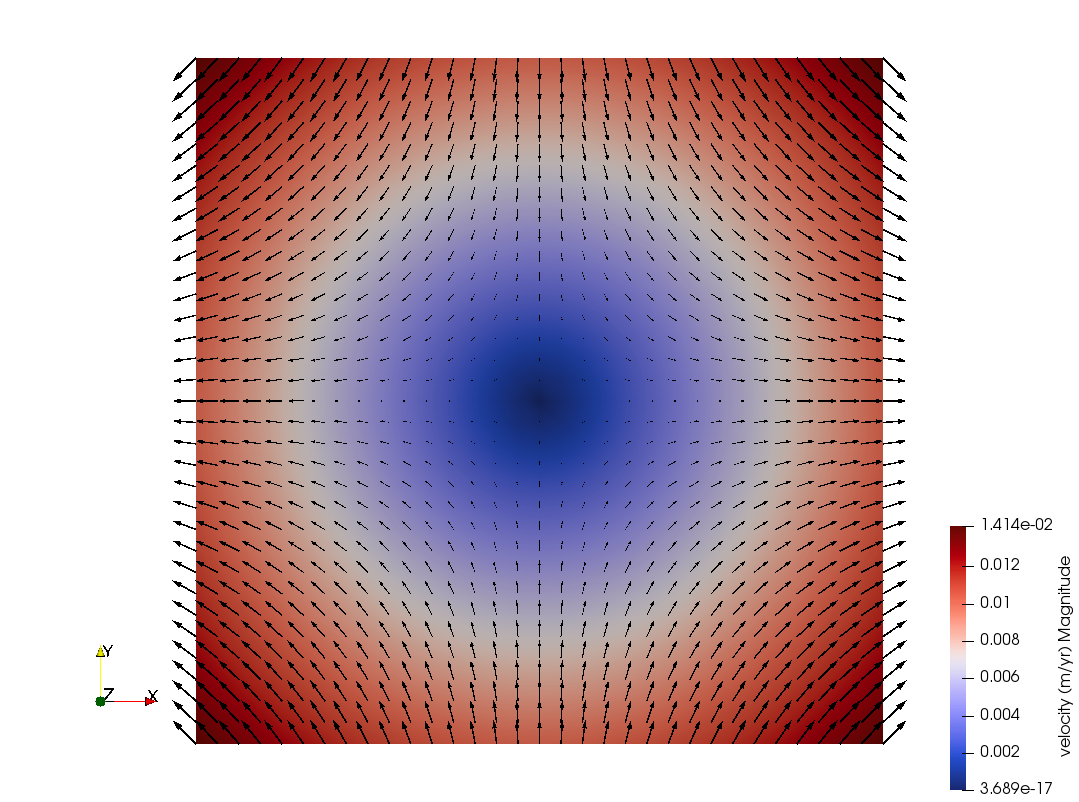
\includegraphics[width=5cm]{python_codes/fieldstone_64/results/buildup/init/vel}
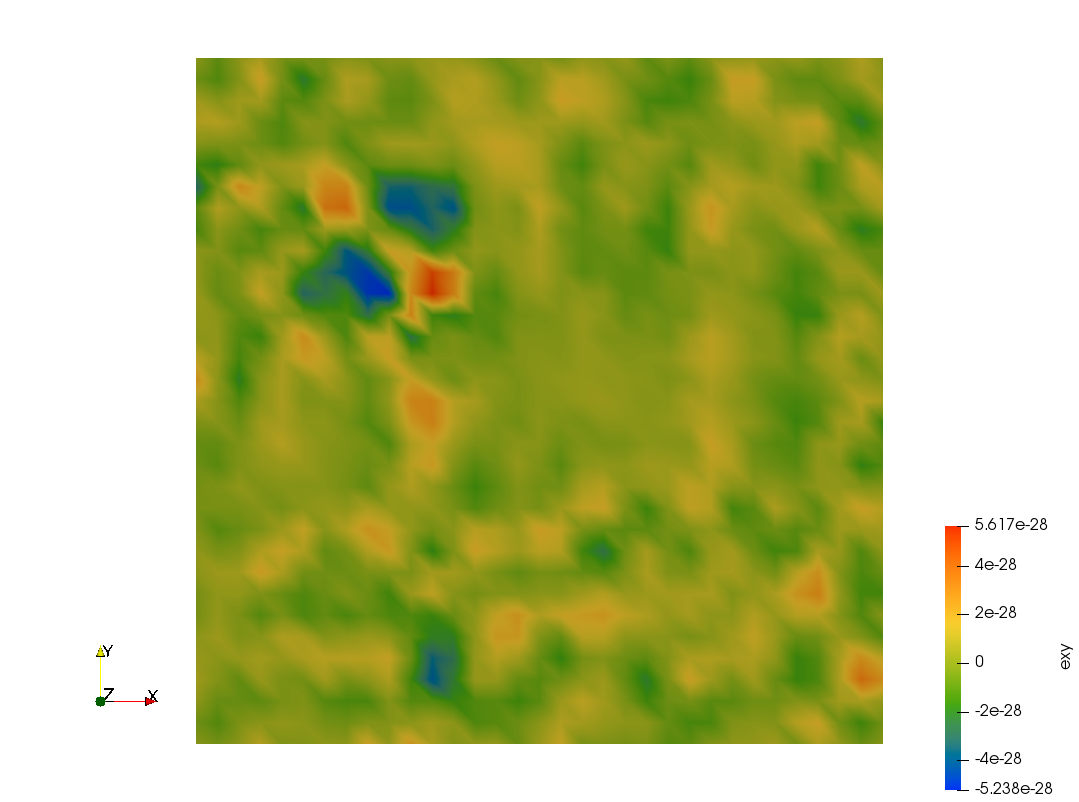
\includegraphics[width=5cm]{python_codes/fieldstone_64/results/buildup/init/exy}
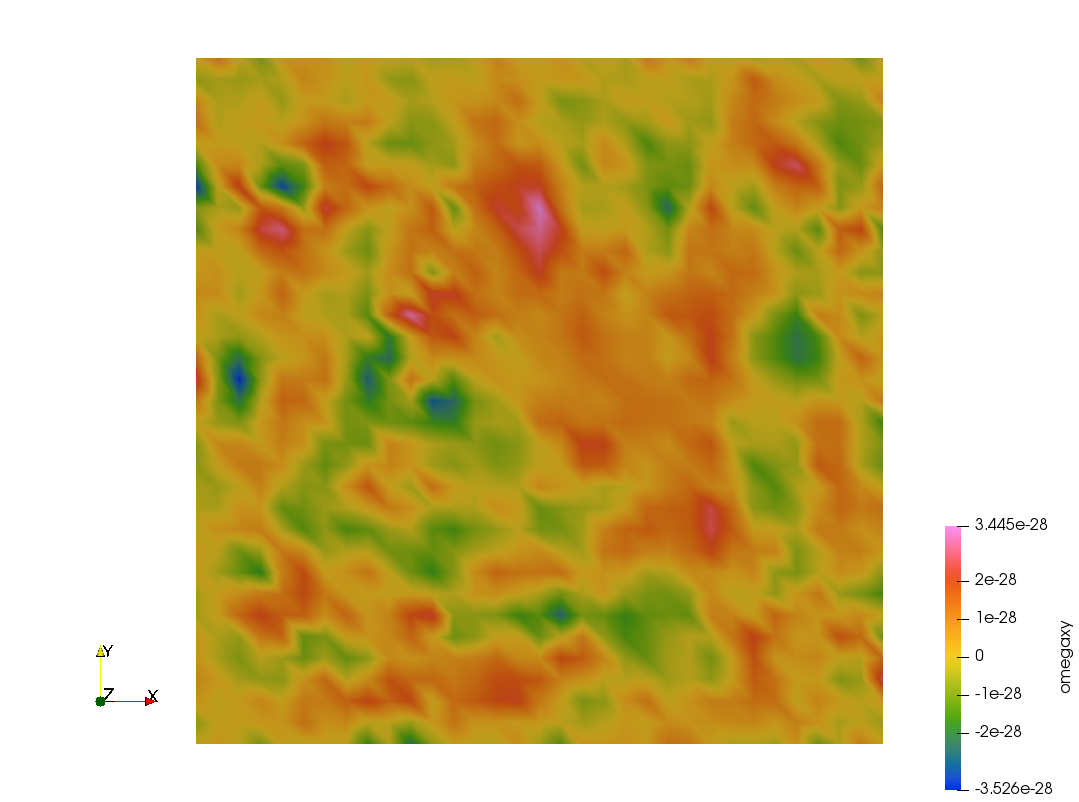
\includegraphics[width=5cm]{python_codes/fieldstone_64/results/buildup/init/oxy}
\end{center}

The expected stress value for $\tau_{xx}$ is 
\[
\tau_{xx} = 2 \eta_{eff} \dot{\varepsilon}_{xx} 
= 2 \cdot 3.057\times 10^{19} \cdot 6.342\times 10^{-15} 
\simeq 38.775 \times 10^4 \text{Pa}
\]

\begin{center}
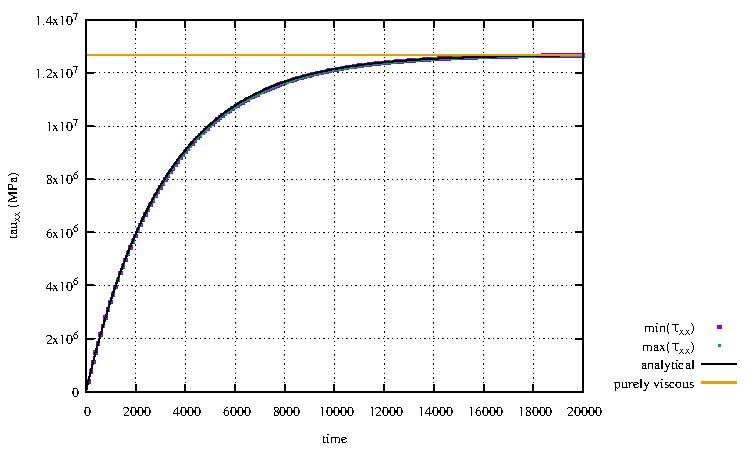
\includegraphics[width=9cm]{python_codes/fieldstone_64/results/buildup/tauxx}\\
{\captionfont $\tau_{xx}$ as a function of time.}
\end{center}



%........................
\paragraph{Bending of elastic slab}

The sinking slab benchmark consists of a beam of elastic material which is placed 
in a weak and viscous surrounding medium. The initially unstressed beam is attached 
to the left domain boundary through boundary conditions. A stress is then applied to 
the beam in the form of gravity. The applied gravity force results in the deformation 
of the beam through bending. After 20 kyr, the gravity field is turned off and the 
elastic properties of the beam will then force itself to its original position.  
The set-up of the benchmark is given in the following figure: 

\begin{center}
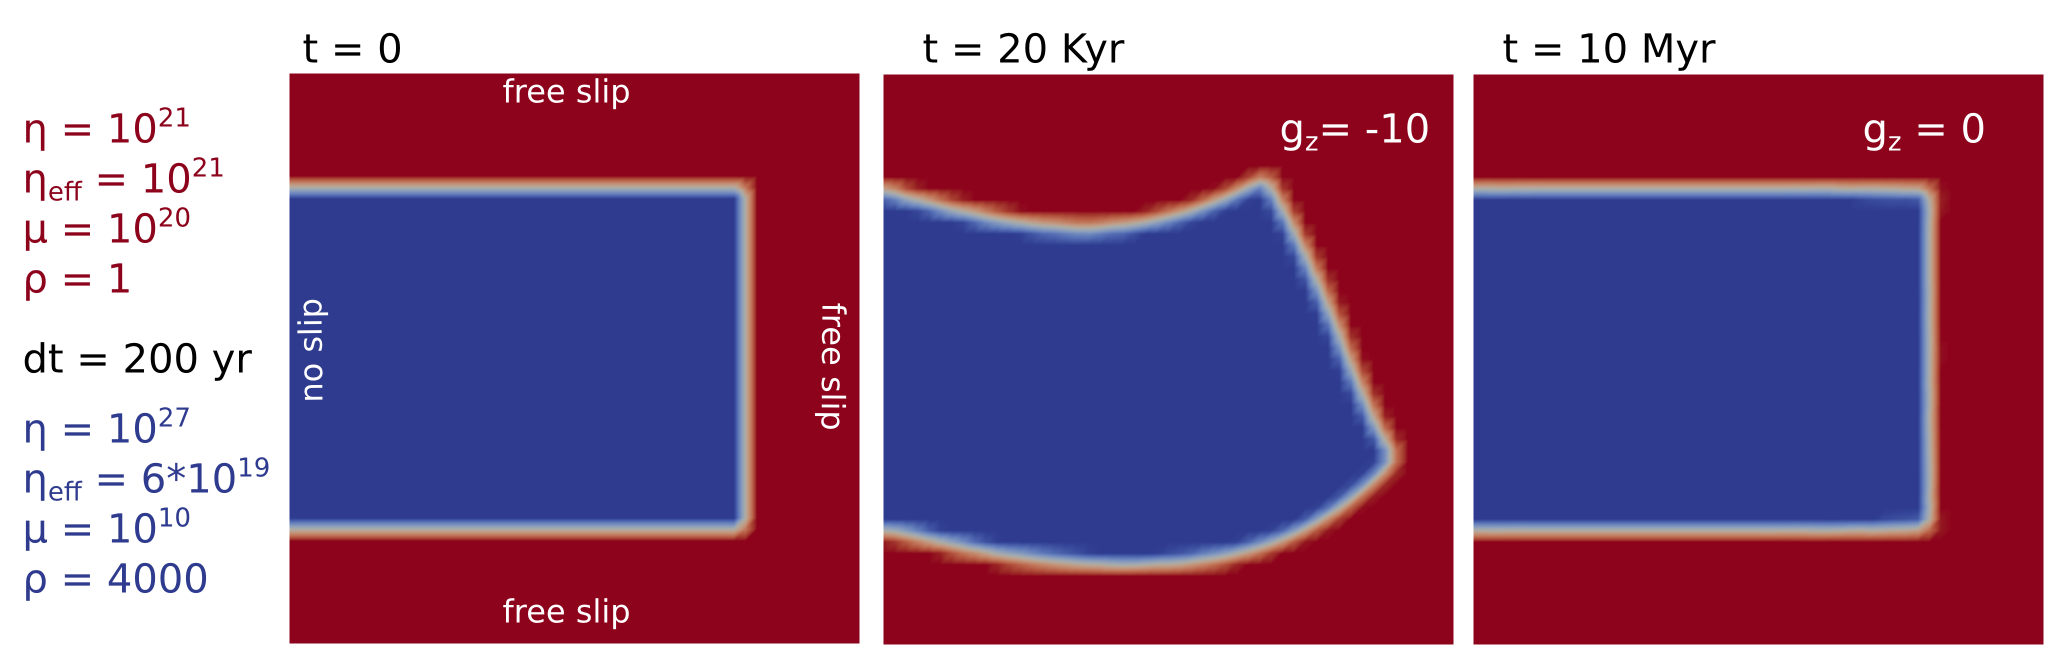
\includegraphics[width=6cm]{python_codes/fieldstone_64/images/poster_benchmark.png}\\
\captionfont{Set-up of the benchmark from \cite{gery10}. The properties of the 
two materials are given on the left, together with the initial configuration of the benchmark.} 
\end{center}

The beam is surrounded by a low-density, low-viscosity and high shear modulus medium 
of which the specifications are given in  the following table.
The boundary conditions of the domain consist of a no slip condition at 
the left boundary where the slab is attached and free slip boundary conditions along all other sides. 
The results are calculated on a grid with a resolution of 50x50 elements.
%The resolution and Courant number will be varied when using compositional fields to see 
%if the models perform better with a higher resolution/lower time step. 
The time step is set to $\delta t = 200yr$.

\begin{center}
\begin{tabular}{lll}
\hline 
\textit{Material properties}& \textit{Elastic slab (fluid 1)}  & \textit{Surrounding medium (fluid 2)} \\
\hline 
\hline 
Density         $\rho$ \     [kg/m$^{3}$]      & 4000                    & 1     \\
Viscosity       $\eta$ \    [Pa$\cdot$ s]      & $10^{27}$               &   $10^{21}$     \\
Shear modulus   $\mu $ \    [Pa]               & $10^{10}$               & $10^{20}$       \\
Maxwell time $t_M$     \    [yr]               & 3.17Gyr                 &  $3.17\times10^{-7}$yr       \\
eff. visc.      $\eta_{eff}$ \ [Pa$\cdot$s]    & 6.307199602192306e+19   &  9.999999984145105e+20      \\
visco-elasticity factor $Z$      \ [-]         & 0.9999999369280039      &  1.5854895966744522e-09     \\
\hline 
\end{tabular} 
\end{center}

\begin{center}
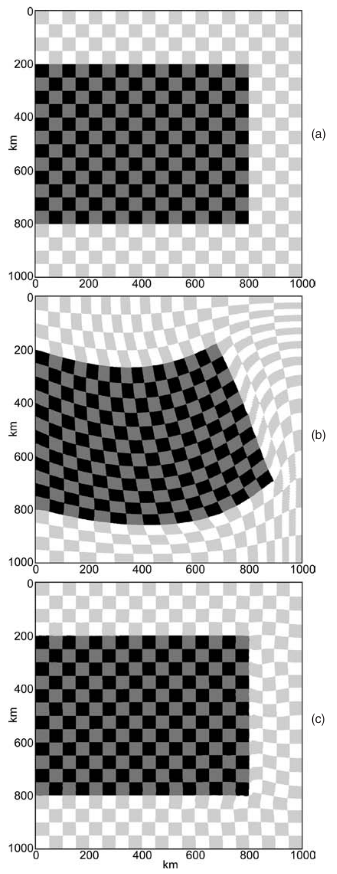
\includegraphics[width=7.6cm]{python_codes/fieldstone_64/images/slabgery10}\\
{\captionfont Taken from \cite[16.11]{gery10}. 
Results of a numerical experiment for the recovery of the original
shape of a visco-elastic slab (black, dark grey), 
 embedded in a weak visco-elastic medium (light grey, white). 
(a) Initial configuration, (b) configuration after 20 Kyr of deformation under 
constant vertical gravity field ($g_x=0$,$g_y =-10\text{m/s}^2$, 
(c) configuration achieved within 9980 Kyr of spontaneous deformation after 
switching off gravity (i.e. after $g_x=g_z=0$ condition is applied at
20 Kyr). Numerical results are calculated at a resolution 51$\times$51 nodes and
200$\times$200 markers. Note the irreversible viscous deformation of the weak surrounding medium,
which is visible in its perturbed checkerboard structure close to slab corners in (c).}
\end{center}

\newpage
The first time that the Stokes system is solved, there is no stored stress, i.e. the 
elastic rhs is identically zero, and the system is solved with a viscosity equal to
$\eta_{eff,1}$ and $\eta_{eff,2}$ for the slab and mantle respectively:

\begin{center}
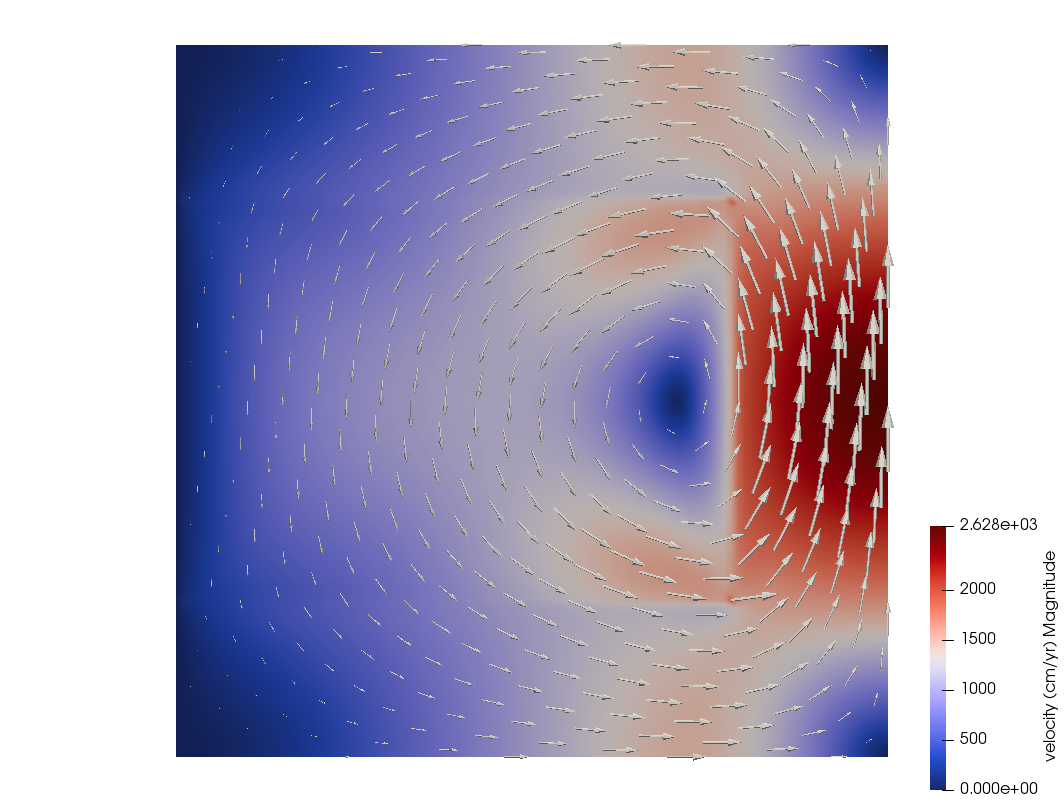
\includegraphics[width=5.2cm]{python_codes/fieldstone_64/results/slab/init/vel}
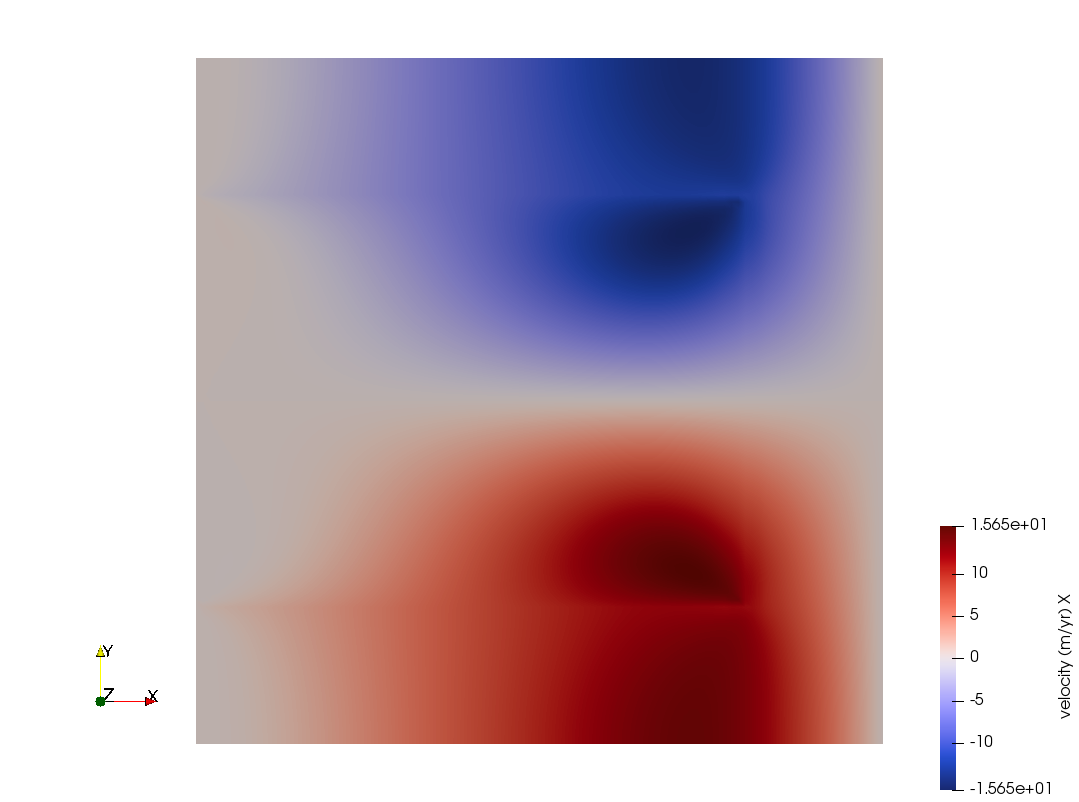
\includegraphics[width=5.2cm]{python_codes/fieldstone_64/results/slab/init/u}
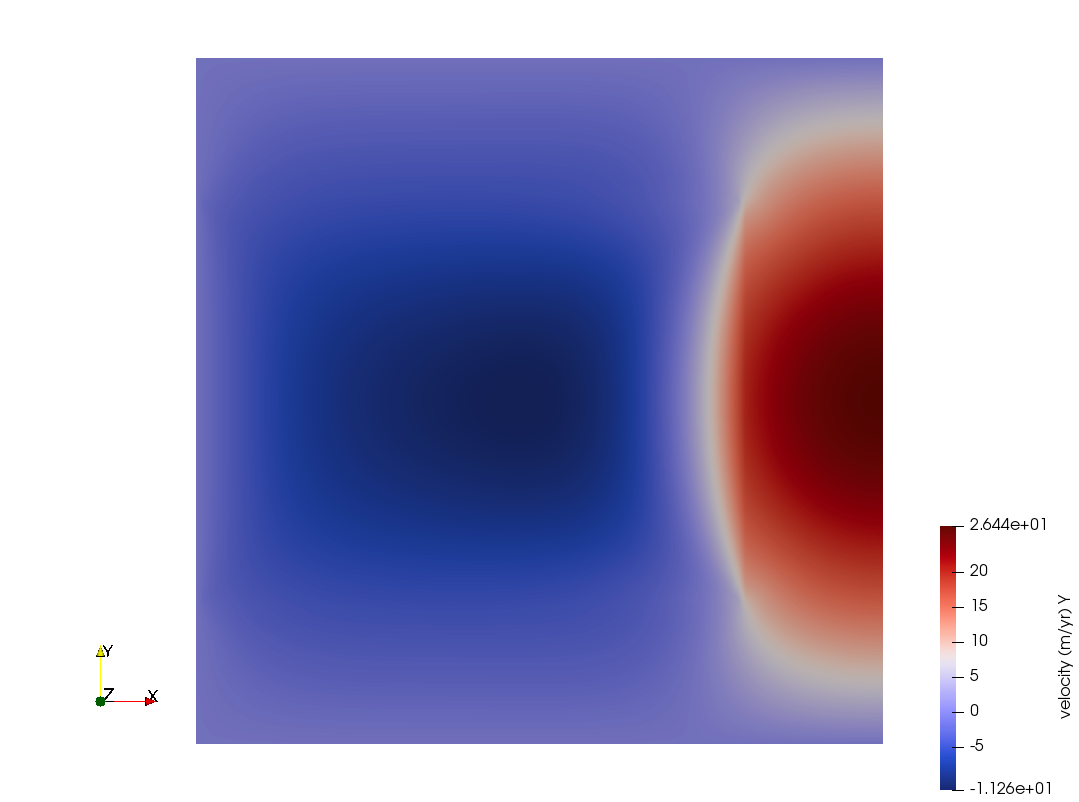
\includegraphics[width=5.2cm]{python_codes/fieldstone_64/results/slab/init/v}\\
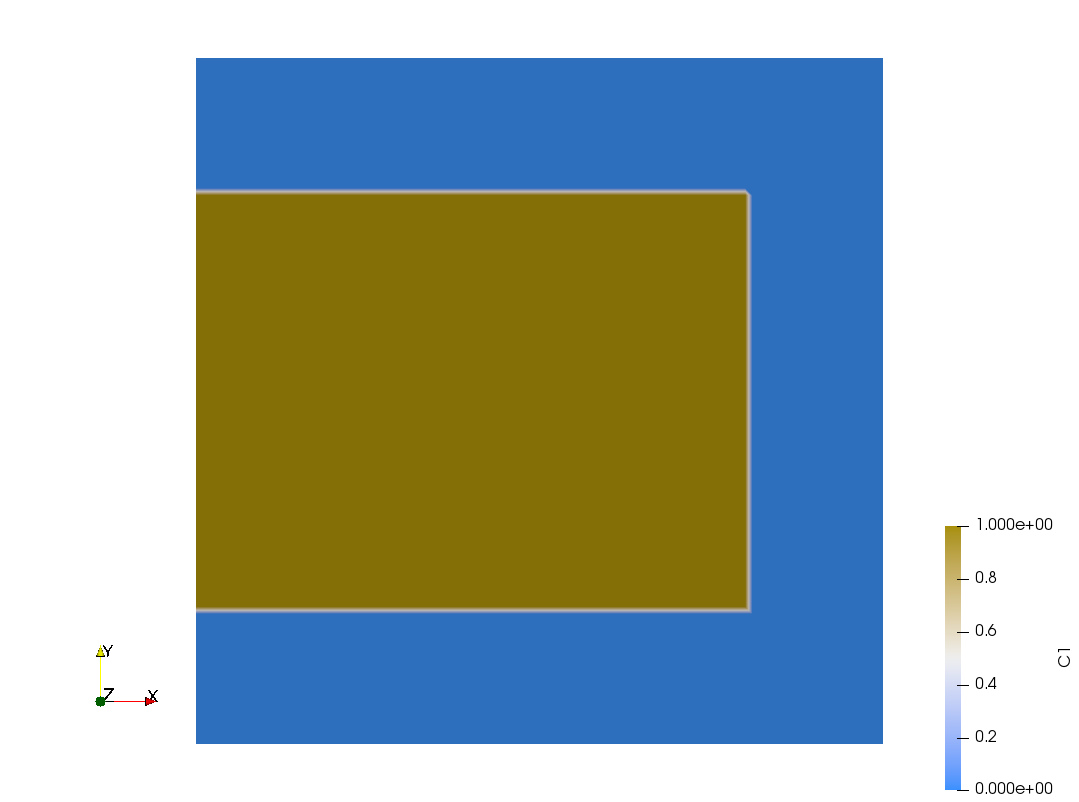
\includegraphics[width=5.2cm]{python_codes/fieldstone_64/results/slab/init/C1}
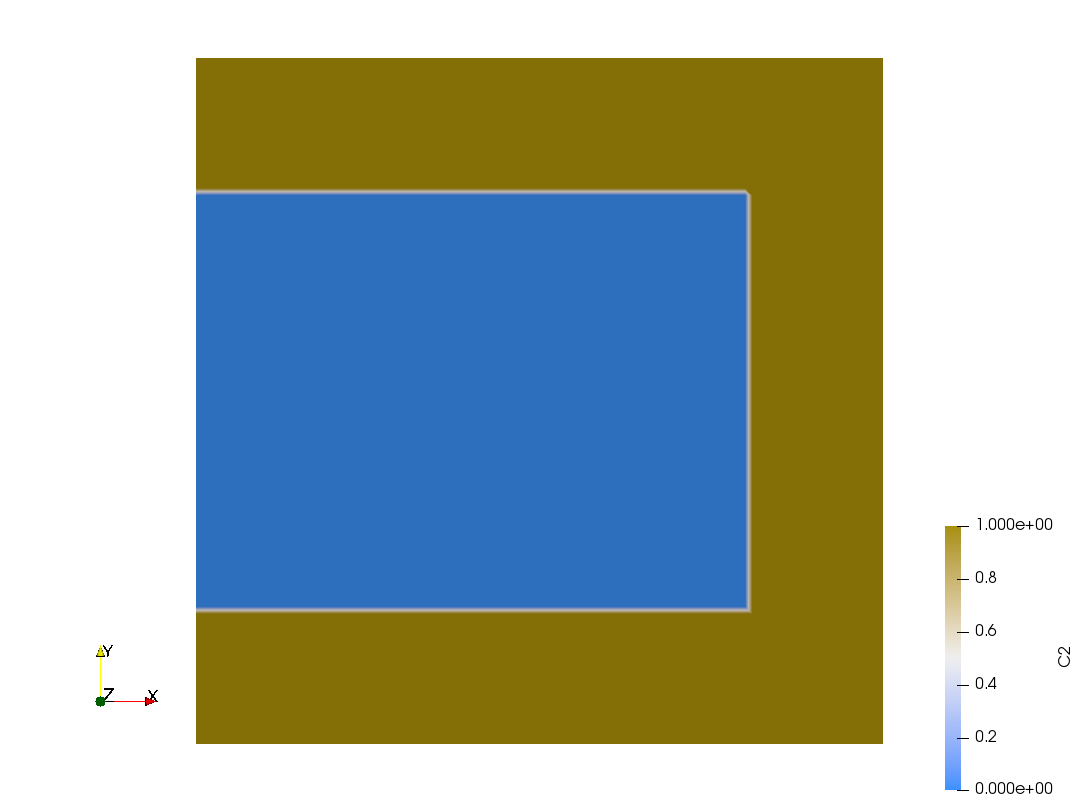
\includegraphics[width=5.2cm]{python_codes/fieldstone_64/results/slab/init/C2}
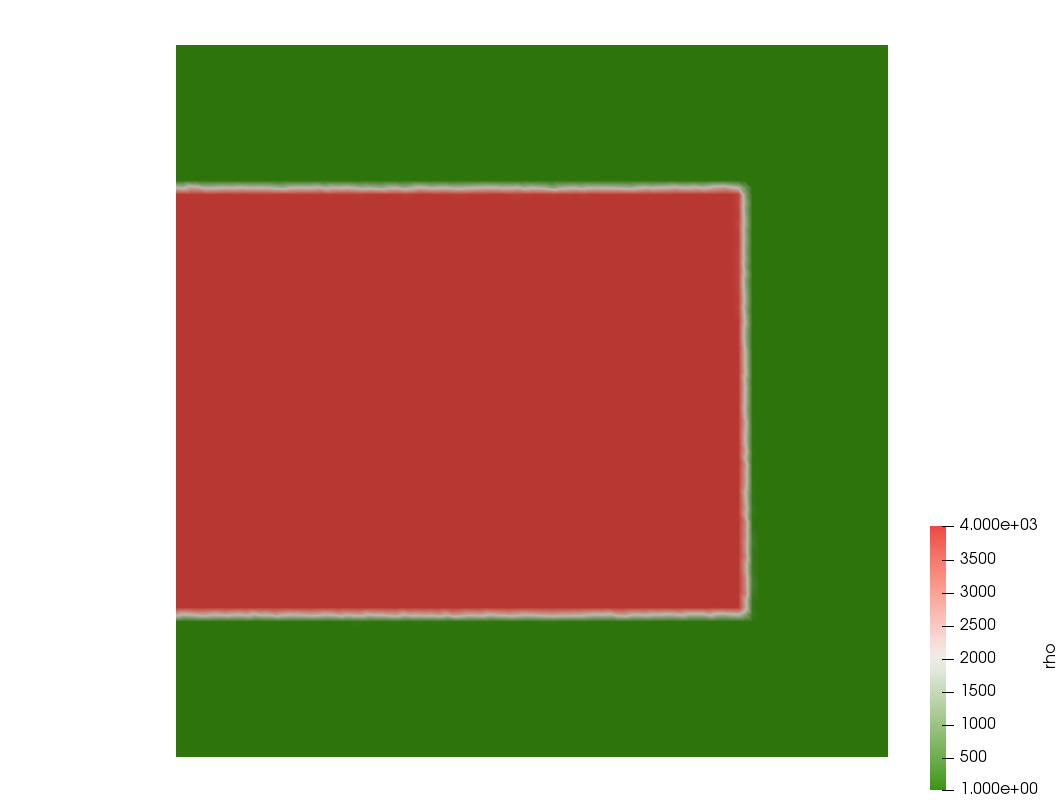
\includegraphics[width=5.2cm]{python_codes/fieldstone_64/results/slab/init/rho}\\
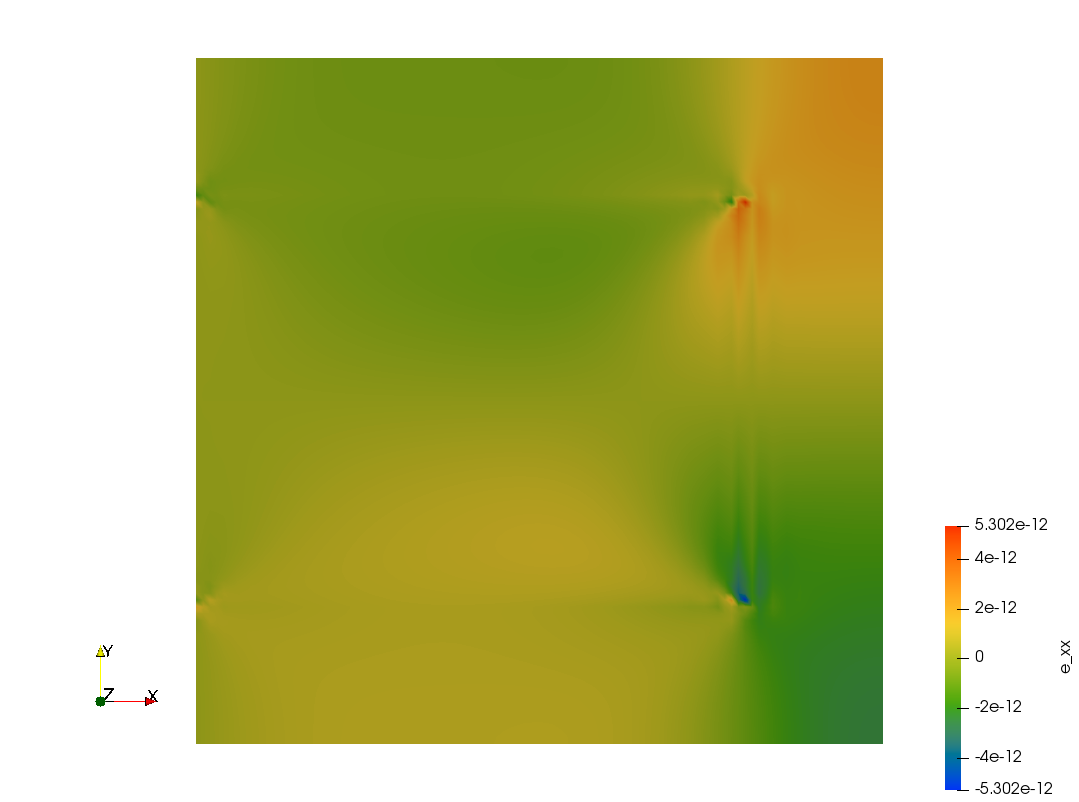
\includegraphics[width=5.2cm]{python_codes/fieldstone_64/results/slab/init/exx}
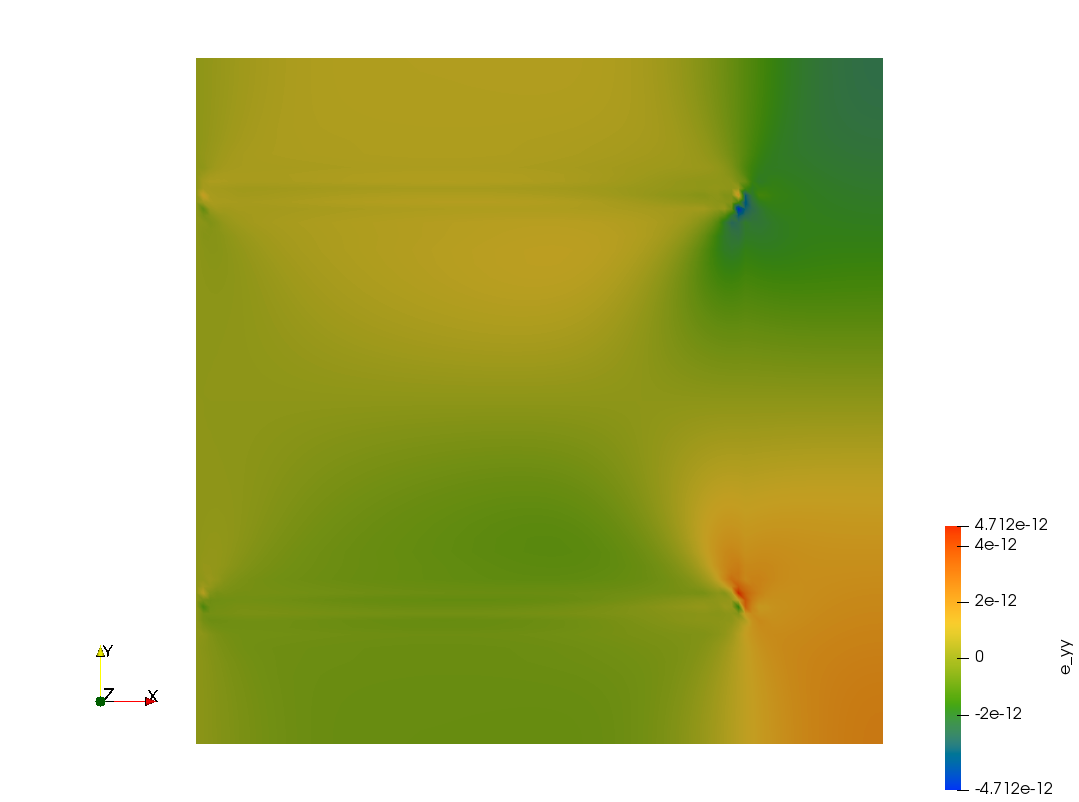
\includegraphics[width=5.2cm]{python_codes/fieldstone_64/results/slab/init/eyy}
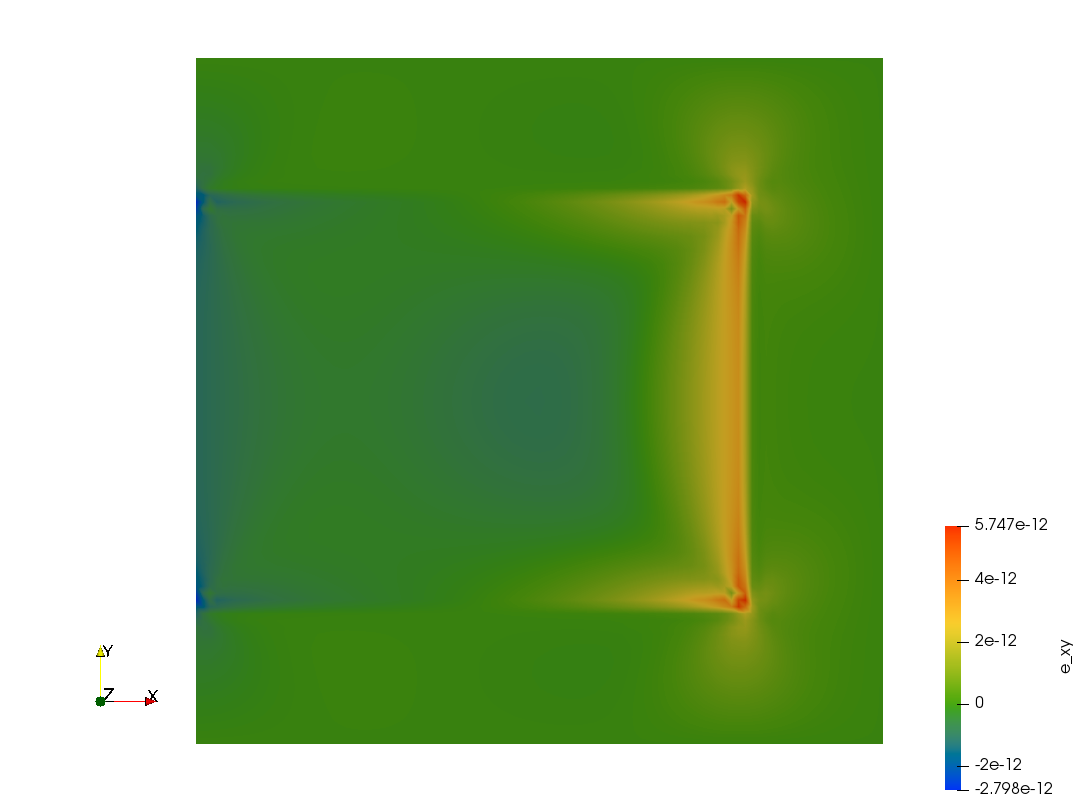
\includegraphics[width=5.2cm]{python_codes/fieldstone_64/results/slab/init/exy}\\
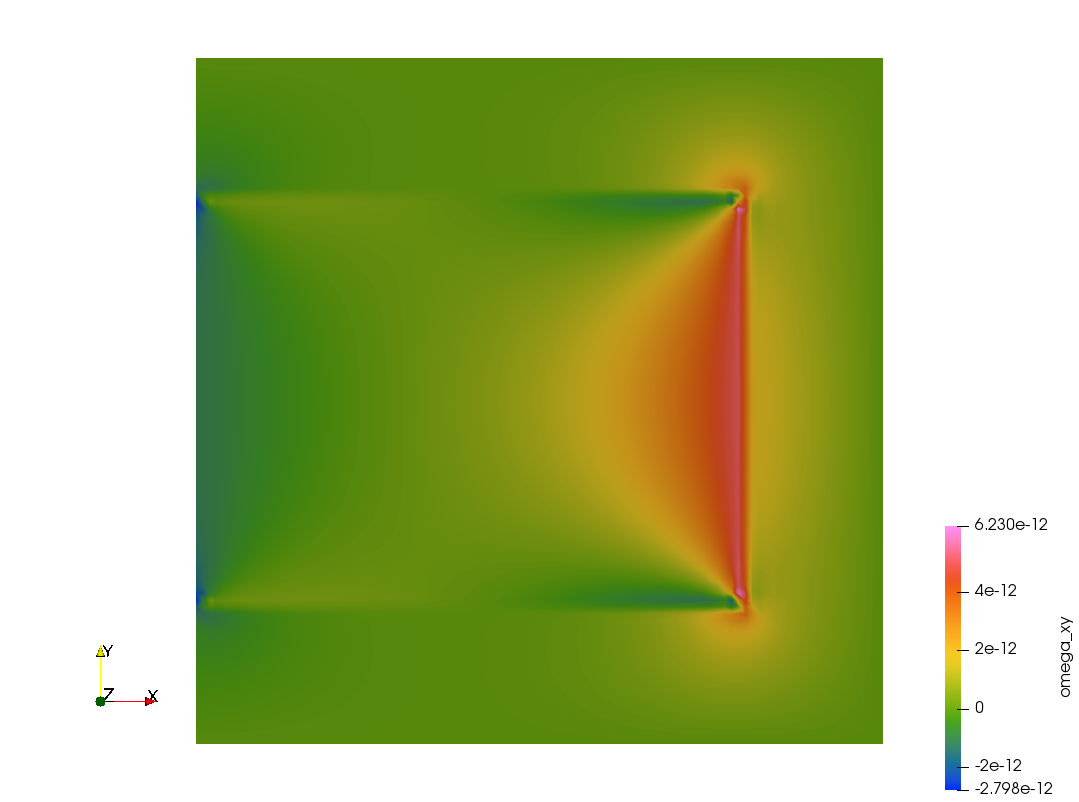
\includegraphics[width=5.2cm]{python_codes/fieldstone_64/results/slab/init/oxy}
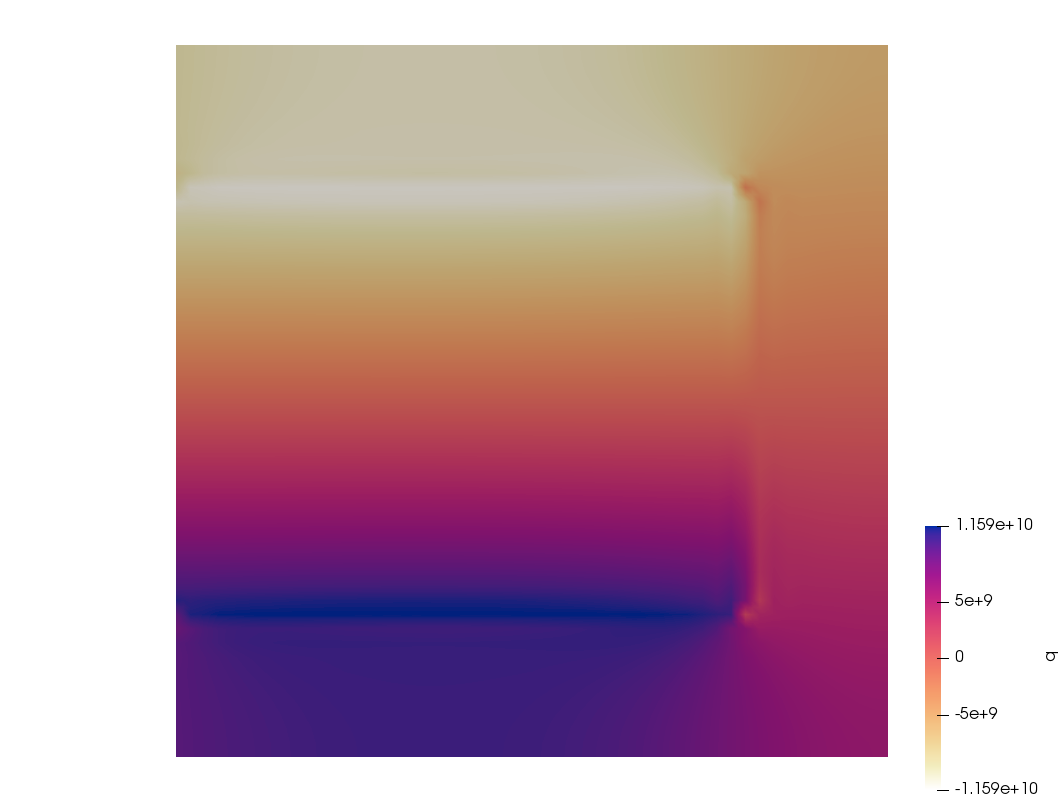
\includegraphics[width=5.2cm]{python_codes/fieldstone_64/results/slab/init/q}
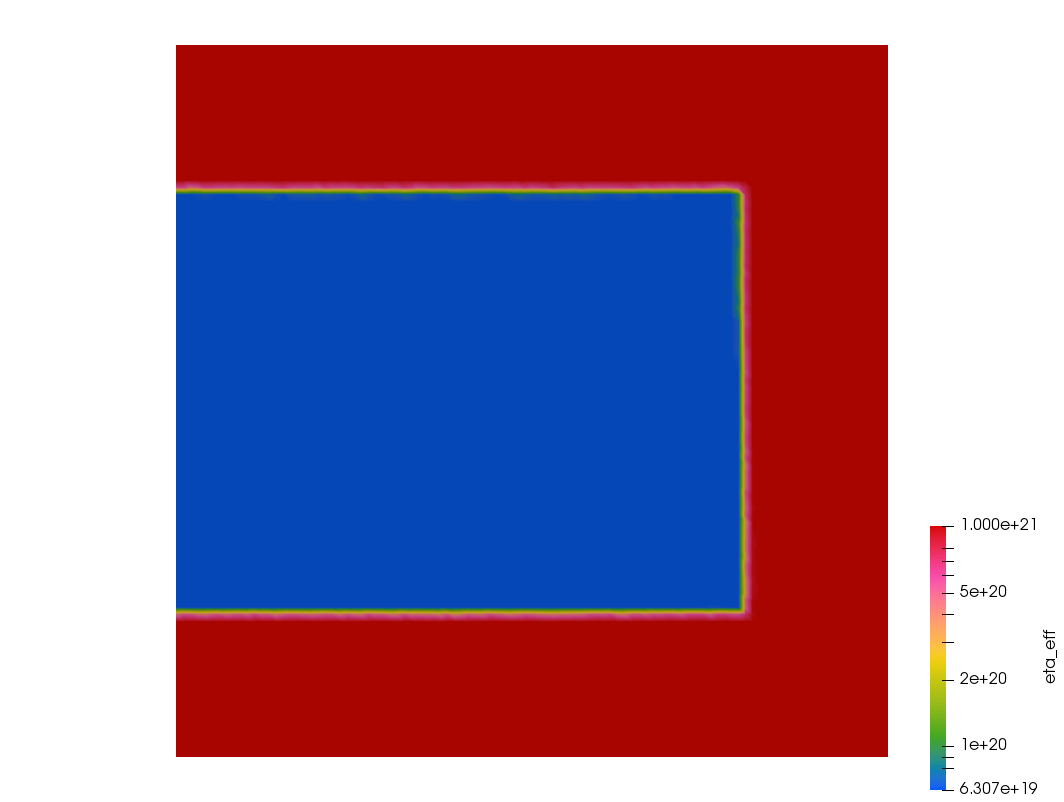
\includegraphics[width=5.2cm]{python_codes/fieldstone_64/results/slab/init/etaeff}
\end{center}

Note that the Gerya data are obtained with the code from the 2010 version of the book.

\begin{center}
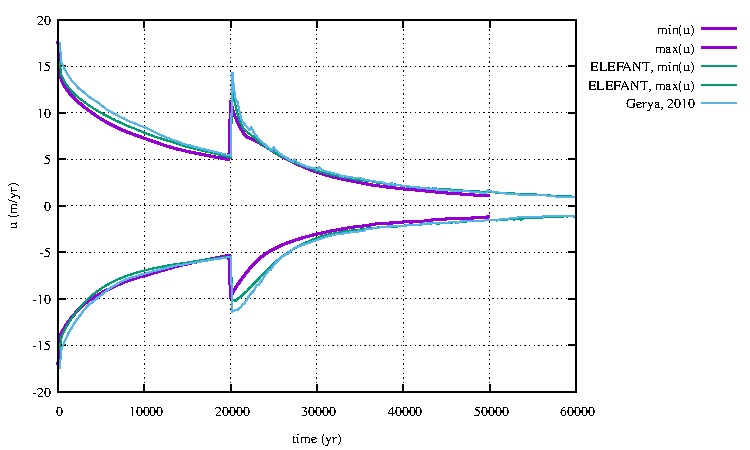
\includegraphics[width=7cm]{python_codes/fieldstone_64/results/slab/velocity_u}
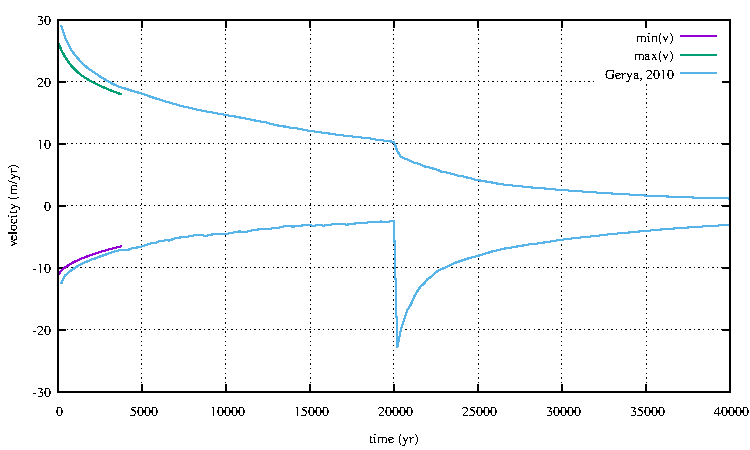
\includegraphics[width=7cm]{python_codes/fieldstone_64/results/slab/velocity_v}
\end{center}


